\chapter{Methods}
This chapter will contain the methodologies applied during the development of this project. Firstly, in section \ref{sec:defprob} there will be the definition of the problem this thesis tries to solve. The selected personality model to be applied in the project is described in section \ref{sec:persmodme}, followed by the explanation of how the data has been collected, in section \ref{sec:datacolme}. Section \ref{sec:baseprojme} introduces the base project, that is the baseline for the artificial agent the algorithms implemented in this thesis are training upon. The description of the gaming algorithm involved will be found in section \ref{sec:mctsmet}, which is a Monte Carlo Tree Search algorithm. Section \ref{sec:mlmethod} includes the probability model in association with our problem. The Genetic Algorithm used to infer information from the dataset can then be found in section \ref{sec:ga}. Lastly, the evaluation of the set of parameters outputted by the above mentioned algorithms can be found in section \ref{sec:meteval}.
\section{Problem Definition}\label{sec:defprob}
The aim of this thesis project is to understand if procedural personæ can be inferred from human game playing, and if it is possible to recreate those personalities by parameters tuning of a Monte Carlo Tree Search algorithm, so to return the optimal move for each state, where optimal in this case means similar to the human player's moves. A set of parameters $\vec{\theta_j}$ would return action $a_j^s$ for a state $s$, while -for the same state $s$- we can expect a different $a_k^s$ for parameters $\vec{\theta_k}$. What we aim to show by the end of this project, is that for a personality $\rho$, we can have a set of parameters $\vec{\theta}_\rho$ that leads the artificial agent to pick the same actions (or equivalent), as a human with personality $\rho$. In order to find the values associated to those set of parameters, we will apply a Genetic Algorithm over the Monte Carlo Tree Search, expecting the optimal set of parameters to match a set of training data.
Finally, each set of parameters $\vec{\theta_\rho}$ will be evaluated on new clusters of data, part of which is of unknown users (with relatively unknown personalities), and part of known testers. The influence that the choice of parameters $\vec{\theta}$ will have on the search outcome, matching or not the correct personality, will confirm or disprove our thesis.
\section{Personality Model}\label{sec:persmodme}
After an extensive research over personality models, the Galen-Hippocrates' model became the best suited for this project, as it seems like different players could be easily mapped to a specific type, giving us some variety and not too subtle distinctions. Furthermore, there is academic background, that gives it some reliability as a model.
Some other models, like BrainHex, or the Big Five, give a more accurate representation of personalities, however the expected amount of data to be retrieved will not give them justice.
Every model listed above could succeed in different settings, but they are either too complicated for our scopes, or they are not backed up by enough academic research to be used as reliable models.
\section{Data Collection}\label{sec:datacolme}
When dealing with Optimization Algorithms and Machine Learning, it is usually suggested to have a discrete amount of data available. Knowing how slow data collection could be, the best option for us would have been to find existing gameplay databases. Unfortunately, as the existing platforms were unresponsive, or the data was just not suitable for our purposes, this research was unsuccessful. Consequently, we set up our own data collection system, taking advantage of the Tiltyard server\cite{tiltyard} as framework. \\
The Tiltyard server has been developed as a testbed for general game players, which also implies it not meant to be strictly used by human players. Because of the not extraordinarily user-friendly interface, we had to provide our testers with an instruction file\cite{datacollection}, as well as a couple of social platforms (a Facebook group and an IRC Channel, to be specific) to find opponents to play against. 
Additionally, in order to keep track of the personalities of the players, we asked our testers to fill a questionnaire with the information not collected by the Tiltyard server, such as usernames, perceived personality of the adversary, and player's own personality.\\
In the instruction file\cite{datacollection}, the testers can find a brief description of the personality models, with a table representation (see table \ref{tab:temperaments}) to help them define their own archetype, the rules of the games, as explained in subsection \ref{subsec:rulesgames}, together with the actual instructions on how to use Tiltyard.\\
To simplify the game set-up process, we have implemented a second version of the Tiltyard homepage, including the choice of playing against the latest version of CadiaPlayer\cite{cadiaplayer, finnsson2007cadia, bjornsson2009cadiaplayer}, a player previously developed at Reykjavik University. However, time constraints have not played in our favour, and the page has not been available to the public early enough to make any actual difference in the data collection process. \\
The participation in the data collection has not been very high, even after organizing periodic events trying to simplify finding an opponent. Only a small amount of games were played in total, but we managed to gather an acceptably uniform distribution of games and personalities, as will be better described in section \ref{subsec:dataresults}.
\subsection{Selected Games}\label{subsec:rulesgames}
The games selected are two players, perfect information games: Checkers, Nine Board Tic-Tac-Toe, Connect Four, and Skirmish. In figures \ref{fig:checkers}, \ref{fig:9boardttt}, \ref{fig:connect4}, and \ref{fig:skirmish} we can see examples of the games while ongoing. Although a few of those games cannot be considered new for our testers, the version implemented in Tiltyard might have included a few variants of the rules as they are traditionally known.\\
The choice of games has been dictated by the list of available games in Tiltyard; once we selected the ones with a usable human interface, we checked the average number of moves.
\subsubsection*{Checkers}
The game is played on a 8x8 squares chessboard, where each player has 12 pieces. The goal of the game is to capture all the adversary pieces by jumping over them. Pieces can move only diagonally, and on unoccupied squares. In this version of the game, capturing is not mandatory, and it is possible to capture multiple pieces during the same turn (if there is an empty square between every two). When a piece reaches the adversary's side of the board, it becomes a “king”, and gains the ability to move backwards. The player who has no more pieces on the board, or cannot move anymore, loses the game (see figure \ref{fig:checkers}).
\begin{figure}[H]
\centering
	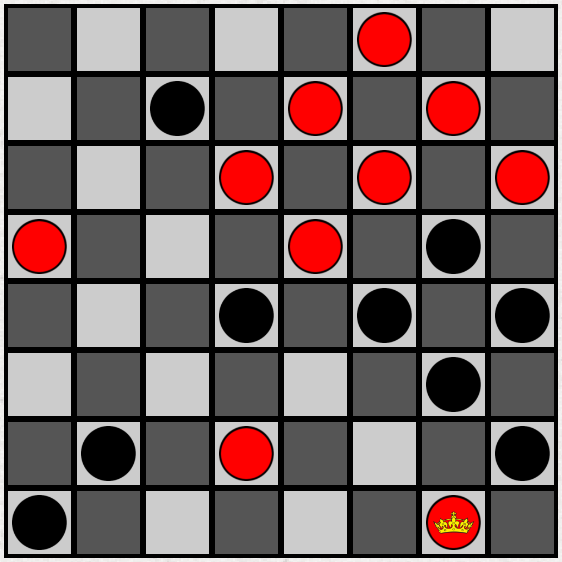
\includegraphics[scale=0.35]{figure/checkers}
    \caption{A game of Checkers.}
    \label{fig:checkers}
\end{figure}
Checkers has been selected because it is a classic game, where non-simple strategies can be developed. It is also the most time consuming game among our choice, having 99.91 moves on average for each game on Tiltyard\cite{checkers}.
\subsubsection*{Nine Boards Tic-Tac-Toe}
The game is played on a grid formed by 3x3 simple Tic-Tac-Toe grids. The first player can play on any board, but his/her choice would force the second player to play in the grid corresponding to the square of the previous move (if player 1 picks the central square, player 2 will have to play in the central grid). If the grid the current player is supposed to play on is full, then any other move is allowed. To win, the player has to win on any one of the boards (see figure \ref{fig:9boardttt}).
\begin{figure}[H]
\centering
	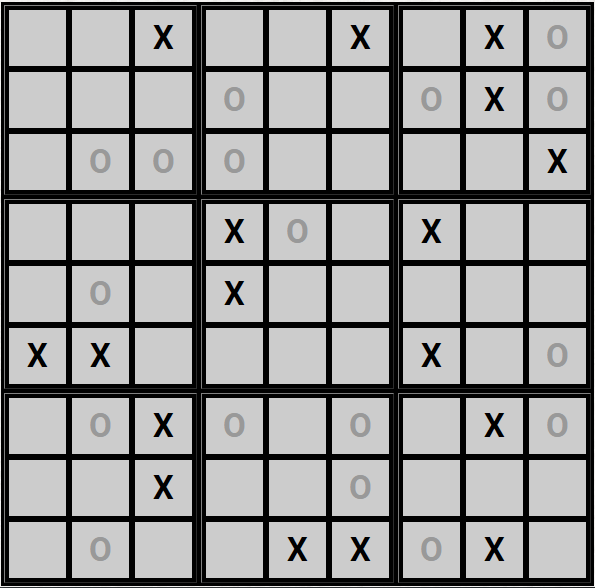
\includegraphics[scale=0.35]{figure/9boardstictactoe}
    \caption{A game of Nine Boards Tic-Tac-Toe.}
    \label{fig:9boardttt}
\end{figure}
Nine-Board Tic-Tac-Toe has 35.07 moves on average on Tiltyard\cite{nineboards}, and has been chosen because it is a variant of the more famous Tic-Tac-Toe, with the advantage of not having the risk of having too obvious moves.
\subsubsection*{Connect Four}
The game is played on a 6x8 suspended grid. Taking turns, the players drop a token of their colour in the grid. The goal is to have 4 tokens connected either horizontally, vertically, or diagonally (see figure \ref{fig:connect4}).
\begin{figure}[H]
\centering
	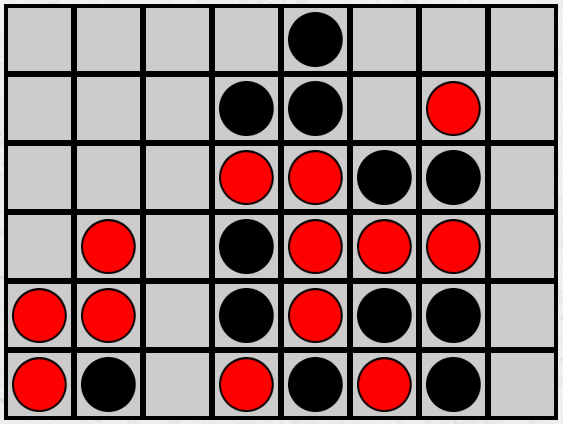
\includegraphics[scale=0.35]{figure/connectfour}
    \caption{A game of Connect Four.}
    \label{fig:connect4}
\end{figure}
Connect Four has been selected for being the "quick game", with only 28.52 moves on average on Tiltyard\cite{connect4}, and being mostly well known worldwide.
\subsubsection*{Skirmish}
The game uses a chessboard and the same pieces as chess, which are also moving in the same way. The pieces are all worth the same, fixed, amount of points -from the pawn to the king-. To win, the player has to eat the most amount of adversary’s pieces. The game terminates when all the pieces of one player have been eaten, or one of the players cannot move anymore. The rules of chess are not rules in Skirmish (i.e. it is not possible to castle, there is no check mate, and so on...), however pawns get promoted to queens when they reach the other side of the chessboard (see figure \ref{fig:skirmish}).
\begin{figure}[H]
\centering
	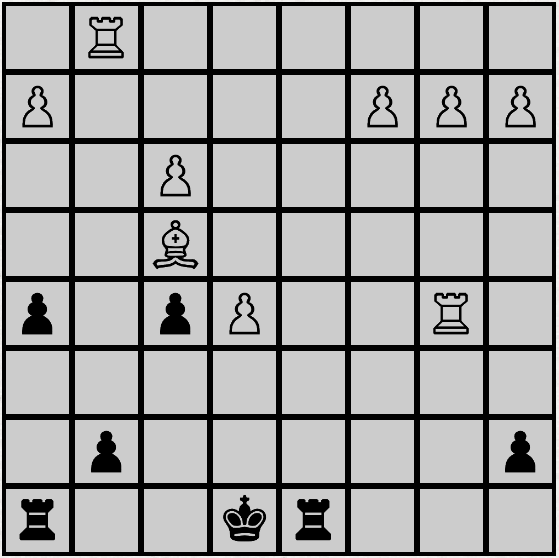
\includegraphics[scale=0.35]{figure/skirmish}
    \caption{A game of Skirmish.}
    \label{fig:skirmish}
\end{figure}
Skirmish has been chosen later in the thesis project, taking the place of another game that had been selected first (called Battle), but was proving to be problematic for our users to play. We then decided that a chess-like game, without falling into the obvious choice of chess, was the perfect game for our evaluation process, having a wide tree search as a consequence of its complexity. Only a handful of matches have been played on Tiltyard, so we do not think that the average number of moves of 59.67\cite{skirmish} is a reliable statistic. 
\section{Base Project}\label{sec:baseprojme}
The implementation of this thesis project has been based on a work with the title of "Virtual General Game Playing Agent"\cite{helgadottir2016virtual}, previously carried out at Reykjavik University. The authors have joined the General Game Playing features with a Unity Player who would mimic human behaviours when playing a game of Checkers or Nine Men's Morris. The player has a virtual reality interface, as we can see in figure \ref{fig:virtualagent}, and it is meant to work with a joystick device and an Oculus Rift. Although the graphic interface is fascinating, we have not taken advantage of it, focusing only on the back-end GGP Engine.\\
\begin{figure}[ht]
\centering
	
\includegraphics[scale=0.3]{figure/virtualagent}
    \caption{A screen-shot of the Virtual Agent while playing a game of Checkers.}
    \label{fig:virtualagent}
\end{figure}
The back-end implementation is based on the ggp-base framework\cite{schreiber2013general}, which provides API for the Game Manager, supplying libraries to handle the GDL reasoner and the communication protocol, to create the game state machines, and to check which moves are legal at each state. This framework has been improved with the addition of a Monte Carlo Tree Search algorithm, tweaked depending on a wide set of parameters that are supposed to give the virtual player a human-like gaming style. Those parameters are the ones that are exploited in the current version of the search, and are described in detail in section \ref{subsec:param}.\\
The Monte Carlo Tree Search is paired with an heuristic dependent on the number of pieces on the board, which would affect the aggressiveness or defensiveness of the virtual player's next moves. However, having a more diverse selection of games in our implementation, we are not adopting the same heuristic, relying on the evolutionary algorithm to find a suitable balance in the 17 control parameters.\\
Lastly, in order to make the virtual agent more human, it has been provided with the choice of a personality. When starting the game, the user can select values to decide which personality the opponent will have. The personality model used here is the Big Five, described in subsection \ref{subsubsec:big5}, and in subsection \ref{subsec:fourvsfive} we can associate the "older" model with the one chosen for the purposes of this thesis' work.
\section{Monte Carlo Tree Search}\label{sec:mctsmet}
The search to evaluate which move needs to be played is implemented as a Monte Carlo Tree Search algorithm with UCT. The algorithm satisfies the requirement of not being game-dependent, and has been giving optimal results in the gaming AI development. In section \ref{sec:mctstheory} we have seen the theory behind it and described the different strategies that can be applied to a basic Monte Carlo Tree Search Algorithm, while in this section we will understand the settings chosen for our purposes.\\
We run our Monte Carlo Tree Search over each game sample, with a set of 17 different parameters that will affect the values in the tree and, possibly, the output. Those parameters could be hand picked and hard coded (as they were in the old project we based this thesis on), or chosen by the evolutionary algorithm described in section \ref{sec:ga}. As mentioned earlier, our algorithm is implemented allowing the addition of RAVE and GRAVE over UCT, MAST, and other enhancements, as early cut-offs, some personality-biased heuristics, and discounting.\\
Our algorithm runs over the matches collected, calculating the QValues for all the moves in each state, but eventually forcefully selecting the same move as the user. This is done to give us an easier way of mapping human behaviour over the states available, focusing only on the knowledge we have available.
\subsection{Parameters}\label{subsec:param}
The Monte Carlo Tree Search parameters are what truly affects the values of each move, as we said earlier. Since each parameter represents and controls a different piece of structure in the search, it is easy to assume that each of them will have its own variable type and a range of meaningful values. More details about the intervals are given in section \ref{sec:ga}. \\
The parameters can be described as:
\begin{itemize}
	\item $Rave$ is the threshold at which only the QValues are considered for selecting moves, and Rave stops being used.
	\item $Grave$ is the threshold setting when Grave stops being used, and only general Rave is used for moves evaluation.
	\item $Charge Depth$ represents the depth limit for a play out.
	\item $Horizon$ represents the maximum depth of the tree.
	\item $Exploration Factor$ is a UCT value that controls the exploration weight over exploitation in the MCTS algorithm.
    \item $Limit$ is the number of simulations the MCTS executes. It has been fixed to be $Limit = 1000$, and will not be modified at any stage during the process.
	\item $Tree Discount$ decides how much discount there is on every move after expanding a node in the tree.
	\item $Charge Discount$ represents the discount applied after each play out.
	\item $Epsilon$ represents the probability of using MAST instead of picking a random move.
    \item $Charge Defaults$ is a couple of default values to be applied if a charge is stopped in early stages.
	\item $Defensiveness$ is a pair of values (one per each player) that bias the goal over valuing defensive moves.
	\item $Aggressiveness$ is a pair of values (one per each player) that bias the goal towards aggressive moves.
    \item $Random Error$ represents the probability of picking a random move instead of the best one.
    \item $Nice Threshold$ biases the move selection, forcing the AI to not always pick the best move and becoming a too strong opponent.
\end{itemize}
The parameters $Defensiveness$, $Aggressiveness$, and $Charge Defaults$ are represented in the search as arrays of 2 items each, one per player. That explains the discrepancy between the number of parameters mentioned earlier, and the number of items in the description list here above.
\section{Probability Model}\label{sec:mlmethod}
In this section the probabilistic model will be described, applying a Bayesian approach. Recapitulating, a set of parameters is plugged into a MCTS algorithm, whose outcome changes the game actions. A dataset of several games where players can be distinguished depending on a personality is given as input. Let a set of uniformly distributed parameters - within different ranges, as described in section \ref{sec:ga} - be defined as $\vec{\theta} = {\theta_1,\ldots,\theta_L}$, where $L$ (where we know $L=17$); $\vec{\rho} = {\rho_1,\ldots,\rho_4}$ indicates any among the people's personalities; and $D_{mcts}^k$ with $k=1,\ldots,M$, is the match data retrieved from the MCTS, where $M$ is the number of matches played. The set of matches associated to a specific personality $\rho$ will be indicated as $M_\rho$. It should also be distinguished from $D_h$, which refers to the human gameplay data that has been collected, with $h=1,\ldots,M$. As a simplification, we will refer to $\rho$ as any of the four personalities, as it is not necessary to singularly specify them in this context, and to $\vec{\rho}$ as the set of all personalities in the model. We refer to Appendix \ref{app:prel} for a brief summary of the probability rules applied in this section.\\
Overall, it is in the interest of this project to confirm the thesis where \begin{equation}\label{eq:thesis}
P(\vec{\theta}) \neq P(\vec{\theta}|\rho), \qquad \forall \rho \in \vec{\rho}
\end{equation} as otherwise we would be proving that the set of parameters $\vec{\theta}$ used will not be relevant to distinguish a common pattern in the behaviour of a user with personality $\rho$. Additionally, it would be favorable that $D_h=D_{mcts}^k,\  \forall h,k \in [1,\cdots,M]$ in other words, it would be optimal to have a set of moves resulting from the MCTS that would match human actions.\\
In figure \ref{fig:BN} is the Bayesian Network representation of the problem, so to help clarify the following statements.
\begin{figure}[H]
\centering
\begin{tikzpicture}[->,>=stealth',shorten >=1pt,auto,node distance=2.8cm, semithick]

  \node[state]	(A)              {$\rho$};
  \node[state]	(B) [right of=A] {$D$};
  \node[state]	(C) [right of=B] {$\vec{\theta}$};

  \path (A) edge	node {} (B)
        (B) edge	node {} (C);
\end{tikzpicture}
\caption{Bayesian Network representation.}\label{fig:BN}
\end{figure}
The goal is to find the probability of $P(\vec{\theta}|\rho)$ over all the set of data, where $$P(\vec{\theta}|\rho) = \int_{1}^{M_\rho} P(\vec{\theta}|D_h^j)P(D_h^j|\rho).$$ Due to the sample-size of our dataset, however, that is equivalent to saying $$P(\vec{\theta}|\rho) = \sum_{j=1}^{M_\rho} P(\vec{\theta}|D_h^j)P(D_h^j|\rho).$$ Starting from the last term of the chain, let $$P(D_h|\rho) = \frac{P(\rho | D_h)P(D_h)}{P(\rho)}.$$ It is assumed that $P(\rho|D_h)=1$ if the personality $\rho$ matches the data $D_h$, or  $P(\rho|D_h)=0$ otherwise. When the dataset matches the personality, it is then obtained that $$P(D_h|\rho) = \frac{P(D_h)}{P(\rho)}.$$ Considering uniform probability over the personalities $\rho$, it is given that $P(\rho)=\frac{1}{4}$, concluding that 
\begin{equation}\label{eq:1}
P(\vec{\theta}|\rho) = \frac{1}{4}\sum_{j=1}^{M_\rho} P(\vec{\theta}|D_h^j)P(D_h^j)
\end{equation} where the matches considered are the one corresponding to the personality $\rho$ considered. The set of games $[1,M_\rho]$ for a specific $\rho$ will from now be referred as $D_\rho$. Rewriting equation (\ref{eq:1}) it is then obtained that \begin{equation}\label{eq:2}
P(\vec{\theta}|\rho) = \frac{1}{4}P(\vec{\theta}|D_\rho)P(D_\rho).
\end{equation}
From equation (\ref{eq:2}) the \emph{posterior} is defined as $P(\vec{\theta}|D_\rho)$, as the probability of having a specific set of parameters $\vec{\theta}$ matching a set of matches $D_\rho={D_h^1,D_h^2,\cdots,D_h^{M_\rho}}$. 
Considering all matches in each set, the probability that needs to be maximised, can be defined as $$P(\vec{\theta}|D_\rho) = \frac{P(D_\rho|\vec{\theta})P(\vec{\theta})}{\sum_{\vec{\theta_j}} P(D_\rho|\vec{\theta_j})P(\vec{\theta_j})}.$$
The problem of maximising the posterior can be reduced to maximising the numerator, as the denominator is the sum over all the possible data and parameters' sets and is constant. Furthermore, $P(\vec{\theta})$ is the \emph{prior} of our model, constant as well, and defined as $$P(\vec{\theta})=\frac{1}{W}$$ where $W$ is the cardinality of the set of all possible parameters $\vec{\theta}$.
Hence, the maximisation problem has scaled down to \begin{equation}\label{eq:argmax}
	\argmax_{\vec{\theta}} P(D_\rho|\vec{\theta})
\end{equation} which happens to be the \emph{likelihood} of the model, where $D_\rho$ indicates all the matches belonging to the same set, defined over a specific personality $\rho$. In other words, it is the probability of selecting a list of certain actions given a set of parameters.\\ Being the games defined as Markov Decision Processes, the likelihood for each match $D_h$ can then be calculated as \begin{equation}\label{eq:likelihood}
P(D_h|{\vec{\theta}}) = P_{\vec{\theta}}(a_1,...,a_T| s_1,...,s_T) = \prod_{t=1}^{T} P_{\vec{\theta}}(a_t|s_t)
\end{equation}
where $T$ is the number of turns in the match, and $P_{\vec{\theta}}(a_t|s_t)$ is the probability of choosing action $a$ in state $s$, in turn $t$. It is to be noted that, on a higher level, multiple actions could be available for selection in any state $s$, due to the non-deterministic policy of the games. \\
The probability of a human player selecting an action $a_{human}$ in a certain state $s$ is calculated using the Boltzmann-Gibbs distribution - which is often associated to multi-armed bandit problems\cite{coulom2006efficient}, hence applicable to MCTS - as $$P_{\vec{\theta}}(a_{human}|s_t) = \frac{e^{Q_{\vec{\theta}}(a_{human},s_t)\kappa}}{\sum_{j=1}^{A}e^{Q_{\vec{\theta}}(a_j,s_j)\kappa}}$$ where $\kappa=0.1$ is a constant, $Q_{\vec{\theta}}(a_{human}, s_t)$ is the Q-value the search with parameters $\vec{\theta}$ has associated to action $a_{human}$ in turn $t$, $A$ is the total of all legal actions at current state, and $Q_{\vec{\theta}}$ is the Q-value of said actions, as calculated from equation (\ref{eq:mcts}).\\
The optimal outcome of the chosen set of parameters for a specific personality would be to have $$P_{\vec{\theta}}(a_{mcts}|s_t) = P_{\vec{\theta}}(a_{human}|s_t)$$ where  in the same state $s_t$, for any state $t \in [1,\ldots, T]$, it is true that $a_{human}=a_{mcts}$.\\
To maximise equation \ref{eq:argmax}, we assume that $P(D_\rho|\vec{\theta})$ can be approximated by the product of $P(D_h|\vec{\theta})$ over all the matches $D_h$ in $D_\rho$, for ease of calculation. That is defined as the fitness function $F(\vec{\theta})$ for the genetic algorithm,  where $\vec{\theta}$ will - in the GA case - be an individual $i$. The fitness is then defined as: \begin{equation}\label{eq:fitnessfunc}
F(\vec{\theta}) = \sqrt[M]{\prod_{m=1}^{M}\sqrt[T]{\prod_{t=1}^{T}P_{\vec{\theta}}(a_{human}^{t,m}|s_{t,m}))}}
\end{equation} where $T$ is the number of turns in each match, $M$ is the number of matches gone through, and, for each state $s$, $a_{human}^{t,m}$ is the action chosen by the human player. It is easy to notice that the fitness function is the geometric mean over all the matches of the probability of selecting the action $a_{human}$ picked by the human player in state $s$. The fitness function uses the geometric mean over the matches in order to normalise the fitness over matches with different number of turns, and the different cardinality of the sets $M_\rho$, for each $\rho\in\vec{\rho}$.
\\The set of parameters $\vec{\theta}$ that derives the likelihood for each set of data $D_i$ is, however, unknown. The optimization method used to find the values applicable to the $\vec{\theta}$ is a Genetic Algorithm with a population of individuals $\vec{\theta}$ and the likelihood (\ref{eq:likelihood}) is utilised as fitness function that needs to be maximised.\\
\section{Genetic Algorithm}\label{sec:ga}
We have tried to solve the optimization problem with the implementation of a Genetic Algorithm, as we previously mentioned in section \ref{sec:gatheory}. \\
We have taken a population of $\Psi=100$ individuals, where each individual has a set of chromosomes $c_i$, where $i=1..17$, representing the parameters of the Monte Carlo Tree Search, described in subsection \ref{subsec:param}, and initialized uniformly at random, in a given interval. Each chromosome's value is allowed to be in a meaningful range, and will be  better described at the end of this section.\\
Each individual is used as parameters to run the search and, once the moves are selected, the fitness $F(i)$ is evaluated as the geometric mean of the Boltzmann-Gibbs distribution function over every turn - or state $s$ - of each match, using equation (\ref{eq:fitnessfunc}) proposed earlier, and repeated here for completeness:
\begin{equation*}
F(\vec{\theta}) = \sqrt[M]{\prod_{m=1}^{M}\sqrt[T]{\prod_{t=1}^{T}P_{\vec{\theta}}(a_{human}^{t,m}|s_{t,m}))}}
\end{equation*} where $T$ is the number of turns in each match, $M$ is the number of matches gone through, and, for each state $s$, $a_{human}^{t,m}$ is the action chosen by the human player. For the GA purposes, $\vec{\theta}$ will be referred to as individual $i$.
Different fitness functions could have been applied in order to possibly find a better fitting one, however, only equation (\ref{eq:fitnessfunc}) has been considered due to time limitations.\\
The selection uses a roulette wheel approach, where each individual has probability $$P(i) =\frac{F(i)}{\sum_{j=1}^{\Psi}F(j)}$$ of being selected, where $F(i)$ is the fitness value of individual $i$. The cumulative probability distribution is then calculated over all the individuals as $$C=\sum^\Psi_{j=1}F(j)$$ and a value $r$ is picked uniformly at random in $[0,1]$. If $$\frac{\sum^{i-1}_{j=1} F(j)}{C}< r < \frac{\sum^{i}_{j=1}F(j)}{C}$$ then $r$ sets the minimum threshold for selecting a specific individual, and individual $i$ is picked. The roulette-wheel method has been preferred over the other selection algorithms, because of its non-biased approach\cite{chipperfield1997introduction}.\\
Taking two selected individuals at the time, we apply crossover with probability $p_c = 0.05$. In case the crossover will not be carried out, the individuals remain unchanged. We will be using averaging crossover, because of its closest analogy with actual genetics\cite{ladkany2012genetic}. Recapitulating, the gene $g$ of the offsprings $o_i$ is derived from the genes of parents $p_i$, and is defined as: $$g_{o_1} = \alpha g_{p1} + (1-\alpha)g_{p2}$$ and $$g_{o_2} = (1-\alpha) g_{p_1} + \alpha g_{p_2}$$ where $\alpha$ is chosen uniformly at random in $[0,1]$ for each gene.\\
Mutation has probability $p_{mut} = 0.1$ to happen, with a creep rate $C_r = 0.4$, which represents the width of the distribution. We are adopting a uniform distribution to apply the creep mutation, so the new gene would be obtained as $$g_m = g - \frac{C_r}{2} + C_r \gamma$$ where $\gamma$ is uniformly distributed between $[0,1]$.\\
The values of $p_{c}$, $p_{mut}$ and $C_r$ have been tuned with few testing over a set of the available games, and have been selected depending on the resulting number of generations, in order to try to avoid premature convergence.\\
The algorithm continues evolving the population, until it becomes stagnant, or one of the individuals reaches an acceptable fitness $f_a = 0.9$. To define a population as stagnant, we first calculate the variance of the chromosomes in all the individuals of the current population, as $$\sigma^2_i = \frac{\sum_{j=1}^{\Psi}\left({\frac{g_j^i-g^i_{\mu}}{\sup(g^i)-\inf(g^i)}}\right)^2}{(\Psi-1)}$$ where $g_j^i$ is the $i$th gene in individual $j$, $g^i_{\mu}$ is the average value for gene $i$, with $i = [1...C]$ and $j = [1...\Psi]$, where $C$ is the number of chromosomes and $\Psi$ is the population size. The population is considered then stagnant when $$max_{i, j}^{C, \Psi}(\sigma_i) <= \sigma_a$$ where $\sigma_a = 0.005$ is what we can consider an acceptable standard deviation for our gene's values pool.\\
When the algorithm stops, the fittest individual will be the best set of parameters to represent the personality of that gameplay set, being it the one with the highest likelihood.
\subsection{Parameters Intervals} This paragraph contains details about the values each gene in the chromosome can possibly take. It is to be reminded that each gene represents a MCTS parameter, as have been described in section \ref{sec:mctsmet}.
The genes are then said to be:
\begin{itemize}
\item long $Rave$, where $Rave \in [0,(y*Limit)]$, with $y$ a small integer constant, and $limit$ the number of simulations the search runs for (for us, $y=5$ and $Limit=1000$);
	\item long $Grave$, where $Grave \in [0, 120]$;
	\item long $Charge Depth$, where $Charge Depth \in [0,100]$;
	\item long $Horizon$, where $Horizon \in [1,20]$;
	\item long $Exploration Factor$, where $Exploration Factor \in [1,UCT_{limit}]$, with \\$UCT_{limit} = \overline{\Lambda_J}+\sqrt[]{\frac{2 \ln n}{n_i}}$, where $\overline{\Lambda_j}$ is the average reward for the state $j$, $n$ is the number of simulation so far, and $n_i$ is the number of simulations after the $i$th move. We can approximate $UCT_{limit}=140$;
	\item double $Tree Discount$, where $Tree Discount \in [0.9,1]$;
	\item double $Charge Discount$, where $Charge Discount \in [0.9,1]$;
	\item double $Epsilon$, where $Epsilon \in [0,1]$;
    \item double[2] $Charge Defaults$, where $Charge Defaults[i] \in [35.00,45.00]$;
	\item double[2] $Defensiveness$, where $Defensiveness[i] \in [0,3]$;
	\item double[2] $Aggressiveness$, where $Aggressiveness[i] \in [0,3]$;
    \item double $Random Error$, where $Random Error \in [0,1]$;
    \item float $Nice Threshold$, where $Nice Threshold \in [0,100]$.
\end{itemize}
The types of the variables refer to Java primitive data types\cite{javadatatypes}, where \emph{long} is a 64-bit two's complement integer, \emph{double} is a double-precision 64-bit IEEE 754 floating point, \emph{float} is a single-precision 32-bit IEEE 754 floating point, and with the notation \emph{[2]} we indicate arrays of 2 elements, or the element of index $i$ if indicated as \emph{[i]}.
\section{Evaluation}\label{sec:meteval}
The evaluation process involves the Skirmish games not used for training, of which we have user-associated personalities, and a set of games from the 2013 and 2014 match archives available on the GGP researchers' website\cite{researchggp}. The archives have been filtered, leaving us with human-played games, with no errors in the match, and that are either completed, or with an acceptable number of moves - to avoid considering games that have been aborted only after a couple of turns. \\ 
Once recovered the winning individuals from the Genetic Algorithm, the evaluation matches are run through both with the correct parameters, and with random ones, calculating the Action Agreement Ratio (AAR)\cite{holmgaard2015monte}, which is the percentage of matching moves between the users' results and the search's. We also calculate $\Delta_Q = Q(a_{human}) - Q(a_{search})$, where $Q(a)$ is the Q-value associated to action $a$ in state $s$. The magnitude of $\Delta$ will be significant to evaluate if the parameters we plugged in are having any influence.\\
The results of the evaluation process will be further discussed in the results chapter \ref{sec:reeval}.